\documentclass[a4paper,oneside,openany,12pt]{memoir}
\usepackage[T1]{fontenc} % To get different font encoding, thus allow \guillemotright.
% Undo bad "side effects" of T1 font encoding (ugly font && chapters in small caps).
% Note that it's now not shown in small caps simply because the selected font does not support it.
\usepackage{lmodern}
\usepackage{graphicx} % For images
\graphicspath{{../gfx/}}
%\usepackage[english]{babel} % For correct word hyphenating.
\usepackage{color}    % For the colored boxes.
\definecolor{LOVDdark}{RGB}{34, 68, 136} %224488 % Why does the "HTML" color model not work?
\definecolor{LOVDlight}{RGB}{240, 243, 255} %F0F3FF % Why does the "HTML" color model not work?
\usepackage{hyperref} % For URLs.
\usepackage{float}    % For custom floats (the info boxes).
\usepackage{wrapfig}  % For floating boxes meant for small notes.
% When loaded before float, doesn't work.
% For figures, maybe not do an frame but a box without border and with background color?
\usepackage[format=hang,font=footnotesize,labelfont=bf,skip=5pt]{caption} % To format captions.

% Include all of this in a separate file!
\newcommand{\HRule}{\rule{\linewidth}{1mm}} % Doet height (zie style) hetzelfde?
\newcommand{\institute}[1]{\gdef\inst{#1}}  % Beamer supplies \institute. We want that, too.
\newcommand{\inst}{}                        % Beamer supplies \institute. We want that, too.
\newcommand{\funding}[1]{\gdef\fund{#1}}    % Provide funding line.
\newcommand{\fund}{}                        % Provide funding line.
\newcommand{\setLOVDversion}[1]{\gdef\LOVDversion{#1}} % Provide the current LOVD version.
\newcommand{\LOVDversion}{}                            % Provide the current LOVD version.

\setlrmarginsandblock{2cm}{2cm}{*} % LEFT-RIGHT
\setulmarginsandblock{2cm}{2cm}{*} % TOP-BOTTOM
\checkandfixthelayout % Without this, nothing works. Took me ages before I found out.
\fixpdflayout % Not sure if we need this, but it was recommended someplace.



%%%%% PAGE HEADERS AND FOOTERS %%%%%
\makepagestyle{LOVD}

% Because we don't have odd or even pages, we only need to define odd pages.
\makeoddhead{LOVD}{\normalfont\leftmark}{}{\normalfont\rightmark}
\makeheadrule{LOVD}{\textwidth}{\normalrulethickness}
\makeoddfoot{LOVD}{}{\normalfont\thepage}{}
\makefootrule{LOVD}{\textwidth}{\normalrulethickness}{\footruleskip}

% Style "plain" is called from chapters. We want chapters to have a footer as well.
\makeoddfoot{plain}{}{\normalfont\thepage}{}
\makefootrule{plain}{\textwidth}{\normalrulethickness}{\footruleskip}

% Additional changes:
\makepsmarks{LOVD}{%
  \nouppercaseheads

  \createmark{chapter}{left}{shownumber}{}{.\space} % (\leftmark) number, followed by a . and a space.
  \createmark{section}{right}{nonumber}{}{.\space} % (\rightmark) no number, (useless: followed by a . and a space).
  % Change "shownumber" to "nonumber" if you don't want the chapter/section number displayed at the header.

%  \createplainmark{toc}{both}{\contentsname}
%  \createplainmark{lof}{both}{\listfigurename}
%  \createplainmark{lot}{both}{\listtablename}
%  \createplainmark{bib}{both}{\bibname}
%  \createplainmark{index}{both}{\indexname}
%  \createplainmark{glossary}{both}{\glossaryname}
  % Might want to keep those, see the manual for further information.
}
% Activate your new pagestyle
\pagestyle{LOVD}



%\newcommand{\maketitle}{%
%  \vspace*{\droptitle}
%  \maketitlehooka
%  {\pretitle \title \posttitle}
%  \maketitlehookb
%  {\preauthor \author \postauthor}
%  \maketitlehookc
%  {\predate \date \postdate}
%  \maketitlehookd
%  \thispagestyle{title}
%}



%%%%% TITLE PAGE FORMAT %%%%%
\setlength{\droptitle}{-3cm} % Moves the title (logo, title, authors etc) 3cm up.
\pretitle{
  \begin{center}
    
\includegraphics[width=17cm]{logo.jpg}
    \vskip 4cm
    \HRule\par\HUGE\bfseries\sffamily} %% Need proper font!
\posttitle{\par\HRule\end{center}\vskip 3cm}
\preauthor{\flushright}
\postauthor{\par\inst\par\vskip 1cm}
\predate{\hfill Last updated } % \hfill aligns the rest of the line to the right. \flushright would have done the same.
\postdate{\par\vskip 2cm \noindent \small \fund}



%%%%% CHAPTER STYLE (CHAPTER HEADS) %%%%%
\makechapterstyle{LOVD}{%
  \setlength\beforechapskip{10pt} % A small distance just above the new Chapter title.
  \setlength\afterchapskip{20pt} % A small distance between the Chapter title and the text.
  \renewcommand{\chapterheadstart}{\vspace*{\beforechapskip}\hrule height 2pt \medskip} % Nice ruler above the Capter title.
  \renewcommand{\chapnamefont}{\normalfont\large\scshape} % CHAPTER
  \renewcommand{\chapnumfont}{\normalfont\huge\bfseries\scshape} % 1
  \renewcommand{\chaptitlefont}{\normalfont\huge\bfseries\scshape} % e.g. "Introduction"
  \renewcommand{\printchaptername}{} % Empty text instead of "Chapter".
                  \renewcommand{\chapternamenum}{ } % Weet niet wat dit anders doet.
                  \renewcommand{\printchapternum}{\chapnumfont \thechapter} % Weet niet wat dit anders doet.
  \renewcommand{\afterchapternum}{. } % Just a dot after the Chapter number, no new line.
  \renewcommand{\afterchaptertitle}{\par\nobreak\medskip\hrule\vskip\afterchapskip} % Nice ruler below the Capter title.
}
\chapterstyle{LOVD}



%%%%% LINK CONFIGURATION %%%%%
\definecolor{linkblue}{rgb}{0.1, 0, 1}
\hypersetup{
  colorlinks,
  citecolor=linkblue,
  filecolor=linkblue,
  linkcolor=linkblue,
  urlcolor=linkblue
}



% The custom floats.
%\floatstyle{ruled}
%\newfloat{infobox}{h!}{floats}
%\floatname{infobox}{}

%\floatstyle{boxed}
%\newfloat{notebox}{h!}{floats}
%\floatname{notebox}{Note:}

% Give all figures a boxed float.
%\floatstyle{boxed}
%\restylefloat{figure}



%%%%% INFOTABLE AND WARNTABLE DEFINITIONS %%%%%
\newsavebox{\infobox}
\newlength{\infoboxlength}
\newlength{\infoboxinnerlength}
\setlength{\infoboxlength}{\textwidth}
\addtolength{\infoboxlength}{-2\fboxsep}
\addtolength{\infoboxlength}{-2\fboxrule}
\addtolength{\infoboxlength}{-1.7cm} % Manually configured value making sure the whole box doesn't exceed the line width.
\setlength{\infoboxinnerlength}{\infoboxlength}
\addtolength{\infoboxinnerlength}{-5pt} % Manually configured value making sure the text doesn't get too near the right border.

\newenvironment{infotable}
  {\begin{lrbox}{\infobox}%
    \begin{minipage}[t]{1.5cm}
      \centering
      \vspace{0pt}
      
\includegraphics[width=1cm,height=1cm]{lovd_information.png}
    \end{minipage}
   \begin{minipage}[t]{\infoboxlength}\vspace{5pt}\begin{minipage}{\infoboxinnerlength}}
  {\vspace{6pt}\end{minipage}\end{minipage}\end{lrbox}%
   \begin{center}
   \fcolorbox{black}{LOVDlight}{\usebox{\infobox}}
   \end{center}}

\newenvironment{warntable}
  {\begin{lrbox}{\infobox}%
    \begin{minipage}[t]{1.5cm}
      \centering
      \vspace{0pt}
      
\includegraphics[width=1cm,height=1cm]{lovd_warning.png}
    \end{minipage}
   \begin{minipage}[t]{\infoboxlength}\vspace{5pt}\begin{minipage}{\infoboxinnerlength}}
  {\vspace{6pt}\end{minipage}\end{minipage}\end{lrbox}%
   \begin{center}
   \fcolorbox{black}{LOVDlight}{\usebox{\infobox}}
   \end{center}}



%%%%% CONFIGURE LEFTBAR (FRAMED PACKAGE) %%%%%
% Taken and adapted from http://tex.stackexchange.com/questions/22526/regarding-the-leftbar-environment
% (thanks, xport & Martin Scharrer)
% I still don't like the space between the bar and the colorbox (can be removed by taking out the \hspace), but
% I want that space *inside* the colorbox.
\renewenvironment{leftbar}[1][\hsize]
{%
    \def\FrameCommand
    {%
        {\color{LOVDdark}\vrule width 3pt \hspace{5pt}}%
        \colorbox{LOVDlight}%
    }%
    \MakeFramed{\hsize#1\advance\hsize-\width\FrameRestore}%
}
{\endMakeFramed}



%%%%% CONFIGURE IMAGES %%%%%
\definecolor{shadecolor}{RGB}{240, 243, 255} %F0F3FF
%\newlength{\imagewidth}
%\setlength{\imagewidth}{\textwidth}
%\addtolength{\imagewidth}{-2\FrameSep}
%\addtolength{\imagewidth}{-2\FrameRule}





%%%%% SETTINGS FOR THE TITLE PAGE %%%%%
\setLOVDversion{3.0-beta-10}
\title{LOVD 3.0 user manual \\\vskip 1cm Build \LOVDversion}
\author{Ivo F.A.C. Fokkema}
\institute{Leiden University Medical Center}
\date{2012-11-01} % I guess it's easier to use this as a "Last modified" column.
\funding{LOVD has received funding from the European Community's Seventh Framework Programme\\(FP7/2007-2013) under grant agreement no 200754 - the GEN2PHEN project.}





\begin{document}

\begin{titlingpage} % We don't want the front to count as page 1.
\maketitle
\end{titlingpage}





\hypertarget{toc}{}
\tableofcontents





\chapter{Introduction}

This is the manual for the Leiden Open (source) Variation Database (LOVD) version 3.0.
LOVD 3.0 is a partial rewrite of LOVD 2.0, which first stable release was completed in 2007.
Also, LOVD 3.0 has a greatly improved database model, and includes lots of new features aimed at making LOVD useful for more research environments.
\par
LOVD is designed to provide a flexible, freely available tool for gene-centered collection and display of DNA variations.
LOVD 3.0 extends this idea to also provide patient-centered data storage and storage of NGS data, even of variants outside of genes.
\\
\par
LOVD was developed approaching the ``LSDB-in-a-Box'' idea for the easy creation and maintenance of a fully web-based gene sequence variation database,
that is platform-independent and uses PHP and MySQL open source software only.
The design of the database follows the recommendations of the \href{http://www.hgvs.org/}{Human Genome Variation Society} (HGVS)
and focuses on the collection and display of DNA sequence variations, but it has fully implemented methods for storing complete clinical data as well.
The open LOVD setup also facilitates functional extensions with scripts written by the community.
\\
\par
The development of (then nameless) LOVD started in late 2002, while it was first officially released in January, 2004.
Before that LOVD was only in use by the \href{http://www.DMD.nl/}{Leiden Muscular Dystrophy pages},
as a not-so-modular system with lots of characteristics specific for that website only.
With the official release of LOVD in 2004 the system had become much more dynamic and customizing LOVD was made easy mostly by editing text-files.
\par
In 2004, LOVD became available under the open source license GPL and with the 1.1.0 release most of the text-files had been replaced by online forms
so customizations can be performed through the web interface.
Early in 2005 the \href{http://www.ncbi.nlm.nih.gov/pubmed/15977173}{first LOVD article} was published,
and in 2005 the development of LOVD was more targeted at improving the ease of use of the system.
\\
\par
In 2006 the development of LOVD 2.0 started after the decision was made to rewrite all of LOVD from scratch
to be able to include a long list of upgrade suggestions that were hard to implement in LOVD 1.1.0.
Aimed at modularity and data redundancy, LOVD 2.0 was meant to be a more flexible and more powerful successor of the popular 1.1.0 version
and soon it received the interest of LOVD users eager to try out the all-new version.
\par
With more features being added and bugs fixed rapidly, LOVD 2.0 reached beta stage in April 2007,
after which more and more users started to upgrade their 1.1.0 databases to 2.0.
Finally, in October 2007 LOVD 2.0 reached the stable stage, after which LOVD 2.0 was continuously improved with monthly releases for two years,
after which the releases became less frequent.
LOVD 2.0 is described in the \href{http://www.ncbi.nlm.nih.gov/pubmed/21520333}{second LOVD paper}.
\\
\par
By 2009 it had became clear that although LOVD 2.0 was a great step forward, there were still key improvements to be made.
Since the complexity of necessary changes had become to great to gradually upgrade LOVD 2.0 systems to include these options,
it was again decided to start from scratch writing LOVD 3.0.
This allowed us to redesign the complete data model in full freedom,
although it should still be possible for existing LOVD 2.0 databases to have all data transferred to LOVD 3.0.
\par
LOVD 3.0 adds even more flexibility, allowing users to focus exclusively on sequence variants,
whilst also allowing an exclusive focus on individuals and clinical data, and anything in between.
It will be possible for different submitters to work together cooperatively on the same data.
Searching through the data is improved extensively,
and webservices of many different sources are used to automatically retrieve gene and transcript information.
Also new in 3.0 is full Next Generation Sequencing (NGS) support,
with the ability to import VCF or SeattleSeq formats.
For VCF file imports, LOVD allows for automatic annotation of the variants.
Both formats support the automatic creation of genes and transcripts in the system,
greatly reducing the amount of work required by curators to get LOVD set up for their research data.
\par
LOVD 3.0 reached beta stage in January 2012. Currently, the latest release is \LOVDversion.
Keep an eye on our \href{http://www.lovd.nl/3.0/news}{news page} for the latest information on LOVD 3.0 development.
\\
\par
Where ever you see ``he'' or ``his'' written in this manual, it should read ``he or she'' and ``his or her'' respectively.

\begin{infotable}
Please note that this manual is work in progress.
Since LOVD 3.0 is still under development and the development is the focus of our efforts, most features in LOVD 3.0 are not yet described in this manual.
Also, features described in this manual may become inaccurate or even incorrect in later versions of LOVD 3.0.
Please bear with us while we finish this manual.
\end{infotable}










\chapter{Installing LOVD}

\begin{infotable}
Please note that if you're just going to \emph{use an LOVD installation that already exists}, you do not need to install anything on your computer.
Any web browser that you already have installed, such as Mozilla Firefox, Google Chrome or Microsoft Internet Explorer, will do.
This chapter describes how to install a new LOVD.
\end{infotable}

Installing LOVD is a ``piece of cake''.
%If you just want to try out LOVD to play around with it a bit, we recommend using the (link) LOVD local install CD, which we currently have available for Windows.
%This LOVD local install CD will install LOVD and all necessary software on your computer in just a few minutes with virtually no effort.
%This CD requires roughly 200MB free space on your hard drive.
%For production environments (you intend to publish LOVD on your institution's server) we recommend a manual install, for which you may require help from your system administrator.
However, you might require help from your system administrator, since there are a few dependencies that need to be taken care of first.





\section{Before you install}
LOVD is a web-based software project.
Therefore, installation requires a correctly set-up webserver.
LOVD has been extensively tested with the Apache webserver, but any webserver able to run PHP scripts should suffice.
You'll need PHP 5.1.0 or higher and MySQL 4.1.2 or higher.
LOVD may work with other database platforms, but we are not developing for other database backends.
You are welcome to try other database backends and report the results to us, but we can't provide any support for it.
For more information, see the \href{http://lovd.nl/3.0/faq/software}{FAQ about software needed}.
\par
A suitable server with the necessary software installed is available at virtually all (academic) institutions and countless (commercial) hosting providers.
\\
\par
Before installing LOVD, be sure you have the required credentials for connecting to the MySQL database.
You need a \emph{hostname}, \emph{username}, \emph{password} and a \emph{database name} to be able to install LOVD.
If you are installing LOVD on a remote server, be sure to have the FTP username and password to be able to copy the necessary files to the server.



\subsection{Download \& Extract}
To download LOVD, go to the \href{http://www.LOVD.nl/3.0/}{LOVD website} and click on the ``Download'' tab.
You can download LOVD in two formats; GZIPped TARball and ZIP archive.
The first format is common for Unix and Linux systems while the ZIP archive is popular on the Windows platform.
Usually you will be able to open both formats.
\\
\par
Download the file of your choice and save it to your hard drive.
Now extract the file using GZIP/TAR or ZIP to the desired location.
On a server, common directories may be /var/www on Unix or Linux servers, or C:\textbackslash{}htdocs on a Windows server.
To be sure, consult the documentation of the webserver software you are using.



\subsection{Pre-install Setup}
You will need to rename the standard config file config.ini.php-lovd to config.ini.php and edit it in, for example, a basic text editor.
This is absolutely mandatory, because you will need to enter the MySQL hostname, database name, username and password here.
\par
Please go through the entire config.ini.php file to determine if you need to change any of the other settings.

\begin{warntable}
A .htaccess file is put in the root directory of your LOVD installation protecting the config.ini.php file.
This will prevent the config file from being accessed by others on Apache HTTP servers (if configured properly), the most commonly used webserver.
If you use Apache, please check that your version and configuration support this feature.
Make sure you have the .htaccess file into your LOVD directory, on Unix and Linux systems it's a hidden file so it can be missed easily.
For the .htaccess file to work, you need to have ``Limit'' and ``Options'' enabled in Apache's ``AllowOverride'' setting.
\par
Also, make sure you have MultiViews or mod\_rewrite enabled. This allows a PHP file like ``/setup.php'' to be accessed as ``/setup''.
\\
\par
\noindent
More information about .htaccess files:\\
\url{http://httpd.apache.org/docs/2.0/howto/htaccess.html}
\\
\par
\noindent
More information about AllowOverride:\\
\url{http://httpd.apache.org/docs/2.0/mod/core.html\#allowoverride}
\\
\par
\textbf{If you use a different webserver}, make sure to configure it to deny access to the config.ini.php file.
LOVD will access the file through the filesystem.
Also, the .htaccess file sets a couple of PHP options and enables mod\_rewrite.
If you use a different webserver, please disable the following PHP options: \emph{register\_globals}, \emph{magic\_quotes\_gpc}, \emph{mysql.trace\_mode}.
Also make sure there is ``MultiViews'' functionality, which allows a PHP file like ``/setup.php'' to be accessed as ``/setup''.%
\end{warntable}





\section{Install process}
To install LOVD on a remote webserver, upload the LOVD directory with all the files to the webserver by, for instance, FTP.
If you install LOVD on your own computer, you do not need to follow this step.
\\
\par
Next, point your web browser to the directory where you've uploaded the LOVD files.
This could, for instance, be \emph{http://localhost/LOVDv.3.0/} or \emph{http://www.your-domain.org/LOVD/}.
LOVD will tell you it's not installed yet, and include a link to the install directory.

\begin{figure}[h]
  \begin{shaded}
  \frame{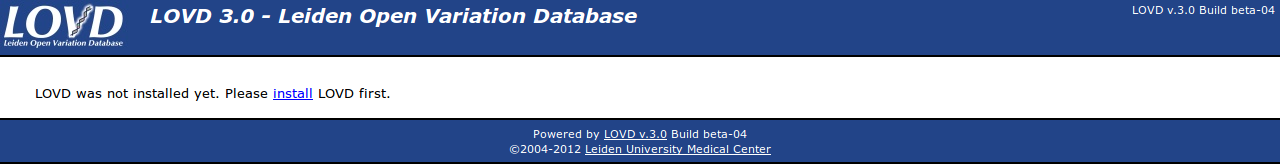
\includegraphics[width=\linewidth]{c02s02_screenshot_not_installed.png}}%
  \caption{%
    When pointing your browser to the LOVD location, it will tell you it's not installed yet.
    Click the link to start the install process.}
  \end{shaded}
\end{figure}

LOVD will first check a few requirements.
Both the PHP and MySQL versions will be checked, to make sure your LOVD will function properly on your webserver environment.
Also some settings of the web server, PHP and MySQL will be checked.
Finally, LOVD will check if your config file has been hidden.
If all looks well, LOVD will tell you all requirements are OK and you're ready to start installing LOVD.
\\
\par
Installing LOVD consists of only 4 simple steps and will take only a couple of minutes, or less.

\begin{figure}[h]
  \begin{shaded}
  \frame{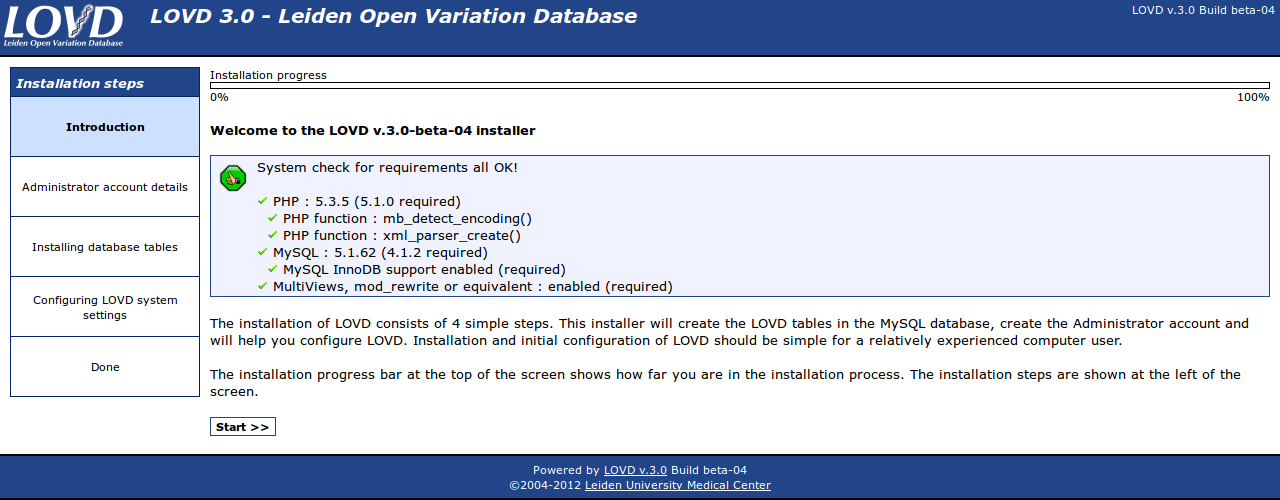
\includegraphics[width=\linewidth]{c02s02_screenshot_installer_01.png}}%
  \caption{If all requirements are OK, you're ready to start installing LOVD.}
  \end{shaded}
\end{figure}



\subsection{Administrator account details}
Fill in the database administrator data to install LOVD.
The database administrator will be the first user registered with LOVD and has full access to all of LOVD's functionalities.
The database administrator is the only user capable of creating manager accounts.
Managers can only create curator and submitter accounts.

\begin{figure}[h]
  \begin{shaded}
  \frame{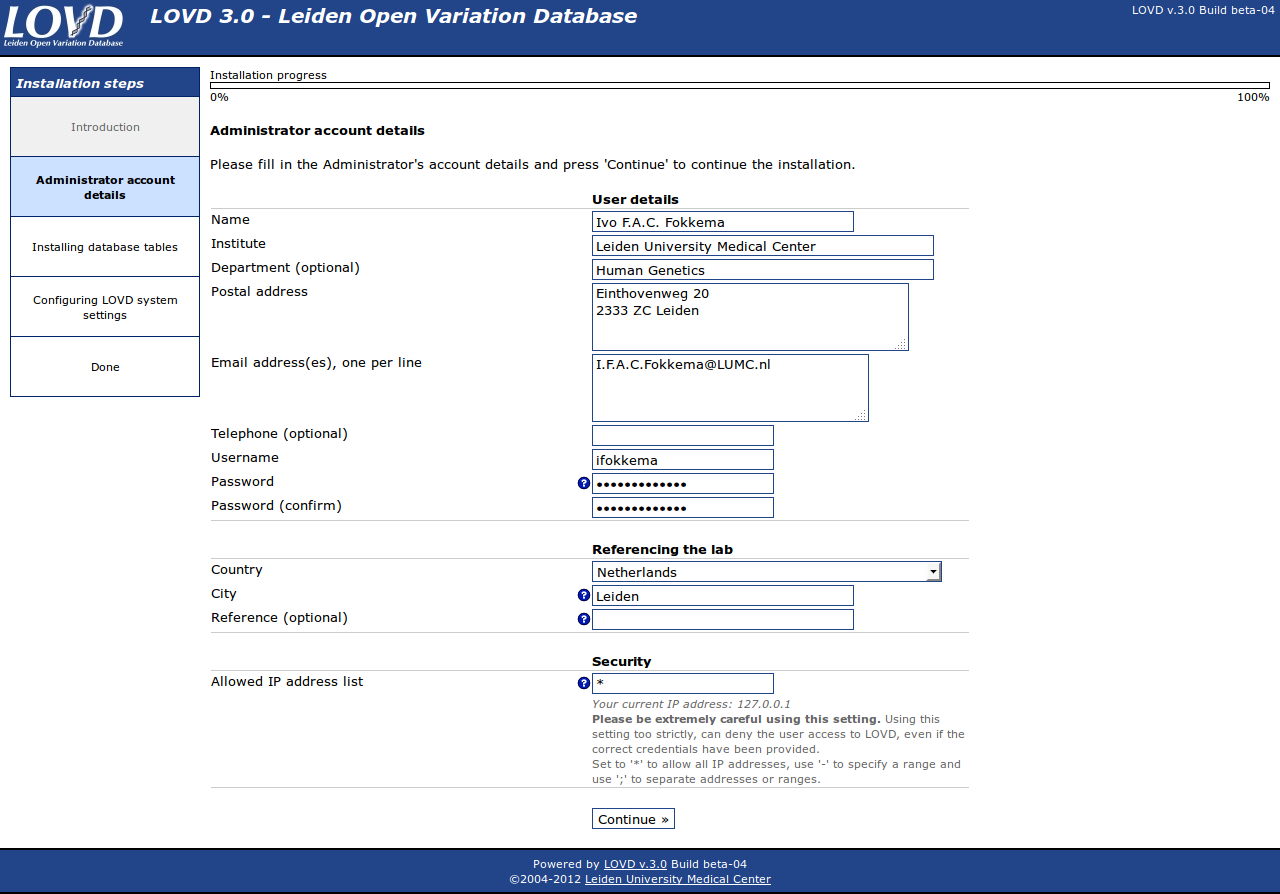
\includegraphics[width=\linewidth]{c02s02_screenshot_installer_02.png}}%
  \caption{The database administrator registration form, with example data filled in.}
  \end{shaded}
\end{figure}

Most of the form is pretty straight forward, but I will highlight one field - ``Allowed IP address list''.
An IP address is an address a computer is known by on the network.
To help prevent others to try and guess the username/password combination,
you can restrict access to the database administrator account to a number of IP addresses or ranges.
This also means you need to be very careful with this setting, as being too restrictive may lock you out of your account.
The default, unrestricted, value is *.

\begin{infotable}
The database administrator is the absolute owner of the LOVD installation.
Not only is he the only one that can uninstall LOVD from the database using the uninstaller,
he will also be able to create, edit or delete all user accounts in the system and
(depending on the settings) receive submission and registration notifications.
\end{infotable}

After completing the database administrator account details, click the ``Continue \guillemotright'' button at the bottom.
LOVD will apply a simple username and password quality check.
If LOVD tells you that the provided details are OK, click the ``Next \guillemotright'' button.



\subsection{Installing database tables}
The next step is to create and fill all necessary LOVD database tables.
LOVD will do this automatically, and you can watch the progress bar complete while the tables are created,
the country list filled, the database administrator account created, the custom columns preconfigured,
the standard columns enabled, and the custom links generated.
This may take a while on non-optimal conditions, so please be patient.
When everything is done, a ``Next \guillemotright'' button appears - click it to continue.

\begin{figure}[h]
  \begin{shaded}
  \frame{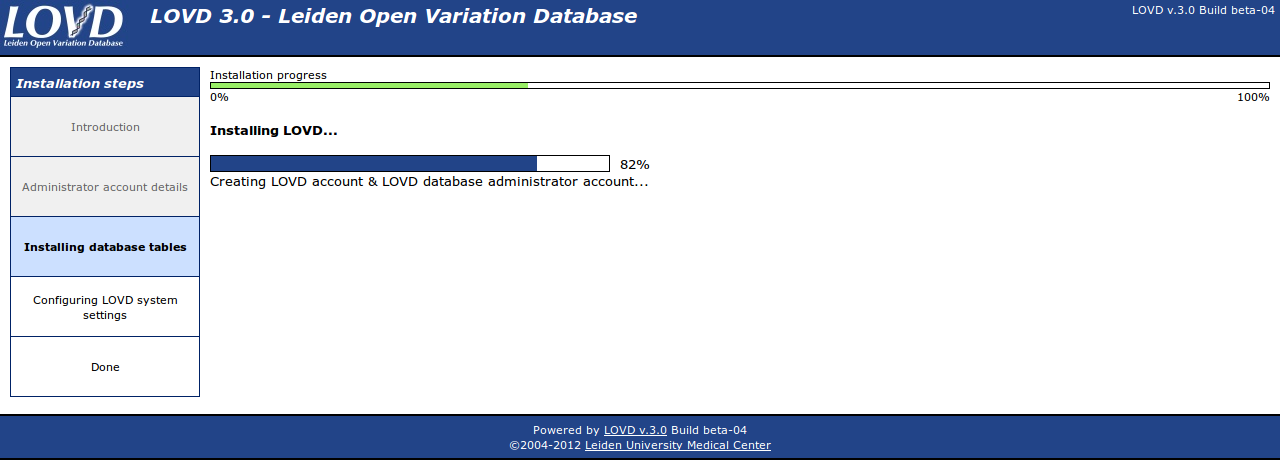
\includegraphics[width=\linewidth]{c02s02_screenshot_installer_03.png}}%
  \caption{Watch the progress bar complete while LOVD informs you which part of the database table installation is currently in progress.}
  \end{shaded}
\end{figure}



\subsection{Configuring LOVD system settings}
The final form in the installation process is completing the initial configuration of the LOVD system settings.
These settings can be changed after installation at any time through the LOVD setup.
\par
The only setting that cannot be changed at a later time, is the install lock, which is checked by default.
Setting the uninstall lock will prevent uninstallation of LOVD by the database administrator.
The only way to remove this lock is directly through the MySQL database backend.

\begin{figure}[h]
  \begin{shaded}
  \frame{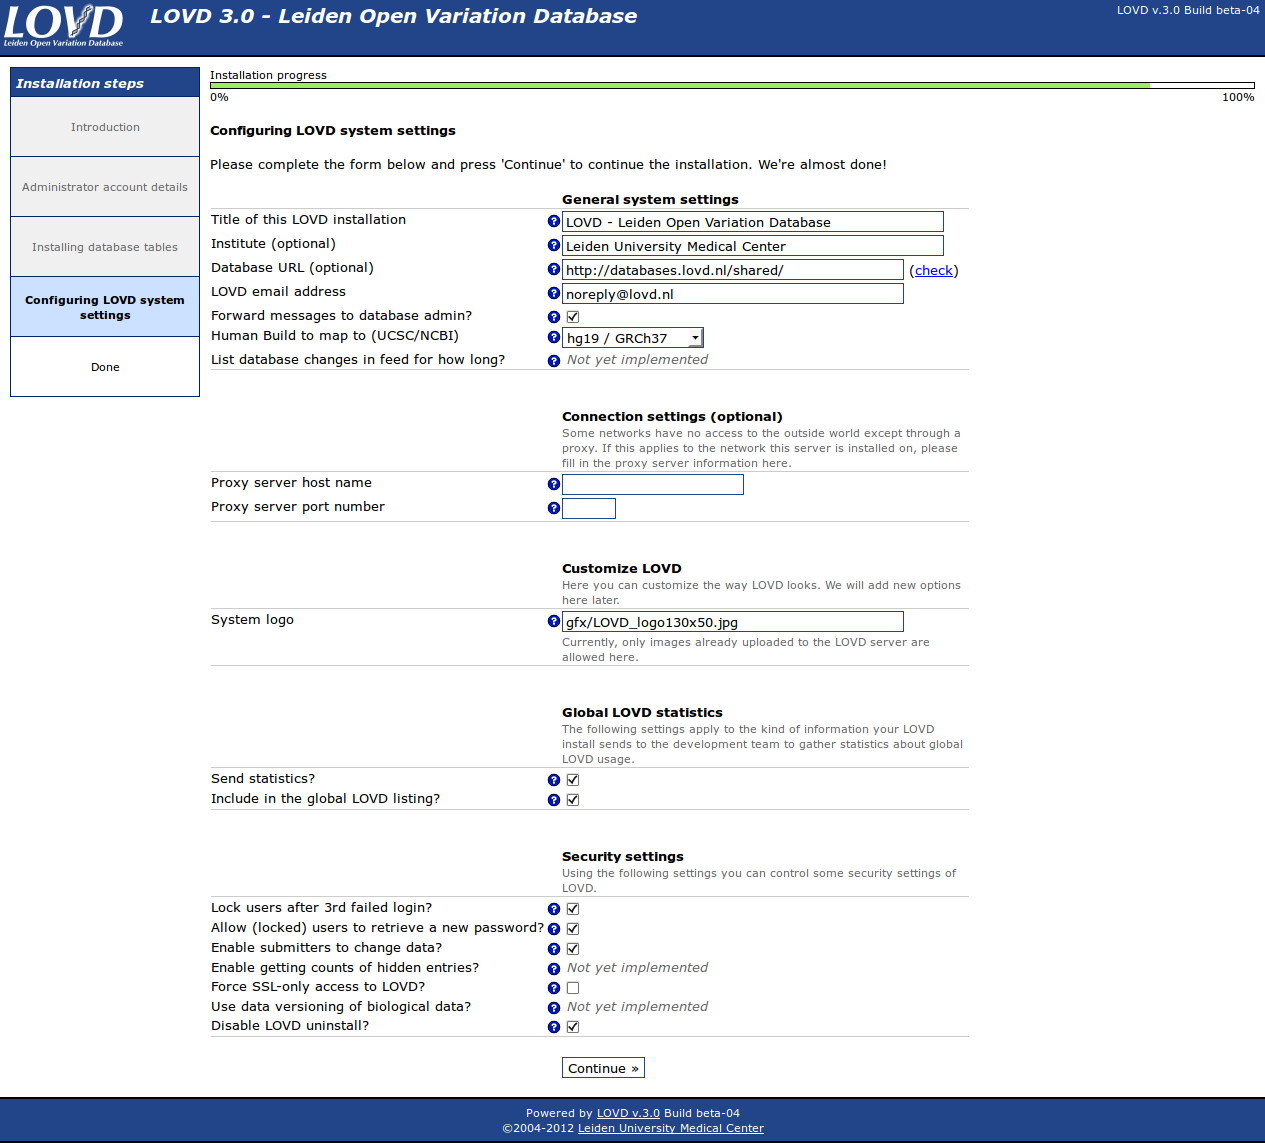
\includegraphics[width=\linewidth]{c02s02_screenshot_installer_04.png}}%
  \caption{The system settings form, with example data filled in.}
  \end{shaded}
\end{figure}

% FIXME
%For more information on the options of the LOVD system settings, see the LOVD system settings section of the manual.
%\\
%\par
After filling in the form, click ``Continue \guillemotright''.
If everything was filled in correctly, LOVD will register the LOVD system settings.
Click ``Next \guillemotright'' to continue to the last step.
Almost done!



\pagebreak[4] % Break the page here (up to 4; 4 is very persistent)
\subsection{Done}
% FIXME; to be honest nothing is done in this step... so... kill it?
When everything has been filled in and stored correctly, the installation is complete.
Now that you're done installing LOVD, click the ``Continue to Setup area \guillemotright'' button to be forwarded to the \hyperlink{c_setup}{LOVD setup area}.
From there, you can perform the most important actions for managers in LOVD, such as creating new gene databases or disease information entries, registering new user accounts or authorizing curators, or manage the custom columns and links.
The button to create a new gene will be highlighted, as a suggestion of your next step!
\clearpage % Makes the hyper target actually point to the right place.










\hypertarget{c_setup}{}
\chapter{LOVD Setup}

To change system-wide settings, but also to perform actions with system-wide effects, start at the LOVD setup area.
The setup area is only available for managers and the database administrator and can be accessed by clicking on the ``Setup'' tab in the menu.
If you do not see a ``Setup'' tab, you first need to log into the system with a manager or administrator account.
\\
\par
The LOVD setup shows some statistics on the left of the screen, like date of installation, number of registered users and variant counts, separated by status.
Furthermore, there are two columns of options.
The left column has options for the system settings, authorized users, the custom columns, custom links, full data download and the LOVD system logs.
The right column has options for genes, transcripts, diseases, individuals and variants.
Some of the general options from the LOVD setup are also available through the Setup tab's dropdown menu, allowing you to quickly navigate to other setup options without having to go through the setup main page.
The other options shown in the setup area are available through their own tab's dropdown menus.
\\
\par
In this chapter, we will describe changing the LOVD system settings, how to check, search and clean up the LOVD system logs, and how to uninstall LOVD.
The other actions available from the LOVD setup are described in their respective chapters (\hyperlink{toc}{see the table of contents}).





% FIXME: I've been trying multiple things to prevent these lists from breaking over one page.
% The most successful was an attempt in creating a new command "\mynobreakpar" that supposedly creates a par that doesn't break.
% The effect was that the text was more compressed (ugly!!!) to try and prevent a broken item, but it still breaks and anyway I just want it to leave space at the bottom of the page instead of compressing everything.
% Writing \nopagebreak in every freaking line is too much, so I checked out "needspace": http://texblog.net/latex-archive/layout/prevent-page-breaks/
% However, \needspace just dumps space there, so if it's not breaking there because of a change of text in front of it, it now shows a big empty part. Ugly, too.
% Now settled for \pagebreak[] commands.
\hypertarget{s_system_settings}{}
\section{LOVD system settings}
\begin{wrapfigure}[3]{r}{8cm} % Only wrap for 3 lines
  \vspace{-25pt}
  \begin{leftbar}
    Required level: Manager\\
    Available from: LOVD 3.0 Build 01
  \end{leftbar}
\end{wrapfigure}
The LOVD system settings allow you to adapt your LOVD installation to your preferences.
For instance by changing the installation's displayed name or email address (general settings), proxy server settings (connection settings), settings on statistics, or the security settings.
\par
To view or edit the LOVD system settings, click on the ``Setup'' tab, then on ``View and change LOVD System settings (...)'',
or move your mouse over the ``Setup'' tab and click the ``LOVD system settings'' menu option from the dropdown list.



\subsection{General system settings}
\begin{description}
  \item[Title of this LOVD installation] \hfill \\
  This title will be shown on the top of every page, above the menu tabs.
  The default value is ``LOVD - Leiden Open Variation Database''.
  \item[Institute] \hfill \\
  The institute which runs this database is displayed in the public area and in emails sent by LOVD.
  It's commonly set to a laboratory name or a website name.
  If it's not specified, LOVD will use the (autodetected) website name LOVD has been installed on.
  \pagebreak[4] % Break the page here (up to 4; 4 is very persistent)
  \item[Database URL] \hfill \\
  This is the URL with which the database can be accessed by the outside world, including ``http://'' or ``https://'', and is not necessarily the URL you are using right now to access the database.
  It will also be used in emails sent by LOVD.
  This field is mandatory if you select the ``Include in the global LOVD listing'' option.
  \\
  If you click the ``check'' link, LOVD will verify or try to predict the value.
  \item[LOVD email address] \hfill \\
  This email address will be used to send emails from LOVD to users.
  LOVD needs this address to prevent problems with spam filters, to make sure that emails from LOVD arrive.
  Please note that although strictly speaking this email address does not need to exist,
  we recommend that you use a valid address to make sure that bounces of emails sent from LOVD (to submitters or curators) are still caught by someone, so that they can be handled.
  \item[Forward messages to database admin] \hfill \\
  With this setting enabled, LOVD will forward messages to the database administrator about submitter registrations, submissions, and such.
  \item[Human Build to map to (UCSC/NCBI)] \hfill \\
  This value can only be set during installation, and cannot be changed later.
  It defines on which version of the Human Build (hg18/Build 36.1 or hg19/GRCh37) genomic variants are described.
  Links to the UCSC and Ensembl genome browsers and the NCBI sequence viewer also depend on this setting.
  \\
  From LOVD 3.0-beta-07, the hg18 setting is no longer available for new LOVD installations, although it will remain to be supported.
  When hg20 will come out, LOVD will start supporting multiple genome builds per installation.
  \item[List database changes in feed for how long?] \hfill \\
  \emph{Note: Not yet implemented!}
  \\
  LOVD includes a ``newsfeed'' that allows users to get a list of changes recently made in the database.
  Select here how many months back you want changes to appear on this list.
  Set to ``Not available'' to disable the newsfeed.
\end{description}



\subsection{Connection settings (optional)}
Some networks have no access to the outside world except through a so-called proxy server (\href{http://en.wikipedia.org/wiki/Proxy_server#Forward_proxies}{more info on WikiPedia}).
If this applies to the network this server is installed on, please fill in the proxy server information here.
\begin{description}
  \item[Proxy server host name] \hfill \\
  The host name of the proxy server, such as ``www-cache.institution.edu''.
  \item[Proxy server port number] \hfill \\
  The port number of the proxy server, such as 3128.
  \item[Proxy server username] \hfill \\
  In case the proxy server requires authentication, please enter the required username here.
  \item[Proxy server password] \hfill \\
  In case the proxy server requires authentication, please enter the required password here.
\end{description}



\pagebreak[4] % Break the page here (up to 4; 4 is very persistent)
\subsection{Customize LOVD}
Here you can customize the way LOVD looks.
Right now, there is only one option included, we will add more later.
\begin{description}
  \item[System logo] \hfill \\
  If you wish to have your custom logo on the top left of every page instead of the default LOVD logo, enter the path to the image here, relative to the LOVD installation path.
  If left empty, it will be set to the default value, which is ``gfx/LOVD\_logo130x50.jpg''.
  Currently, only images already uploaded to the LOVD server are allowed here.
\end{description}



\pagebreak[0] % ``Please'' break the page here (up to 4; 4 is very persistent)
\subsection{Global LOVD statistics}
Your LOVD installation can send some general information on your installation back to us.
We use this information to see how many LOVDs there are worldwide, which versions of LOVD are currently in use, how LOVD is being used (amount of data), to see what type of software is used to run LOVD and to construct the public list of LOVD installs.
\begin{description}
  \item[Send statistics] \hfill \\
  When this setting is enabled, LOVD will collect general usage statistics and send this to us.
  The following information is sent: the number of submitters, genes, individuals, variants and unique variants in your system.
  No specific information is sent, just the numbers.
  \item[Include in the global LOVD listing] \hfill \\ %% FIXME; When LOVD 3.0 site has such a list, use that URL here.
  On our website, we keep a \href{http://www.lovd.nl/2.0/index_list.php}{list of public LOVD installations}.
  This list is also feeding our \href{http://www.lovd.nl/LSDBs}{worldwide LSDB list}, through which submitters can locate databases for a specific gene to submit data to.
  If you enable the ``Include in the global LOVD listing'' setting, your LOVD installation will send us all the information we need to build these lists:
  the LOVD installation's name, the URL, the available gene databases, the date of last update of the gene databases,
  the disease abbreviations and names of the diseases related to these genes and finally the names, institutes and email addresses of the curators of these gene databases.
  If you change this setting, please allow one day for the setting to take effect.
\end{description}



\hypertarget{ss_security_settings}{}
\subsection{Security settings}
In this section you can control some security settings of LOVD.
\begin{description}
  \item[Lock users after 3rd failed login?] \hfill \\
  With this setting enabled, submitters, curators and managers will be locked out of the system after they have provided the wrong password three times.
  A manager or, in the case of a locked manager, the database administrator needs to unlock the user's account once it's locked.
  \\
  This does \emph{not} affect the database administrator account.
  \item[Allow (locked) users to retrieve a new password?] \hfill \\
  If a submitter, curator, or manager has lost his password, enabling this ``I forgot my password'' feature allows them to receive a unlocking code in their email with which they can unlock their account and choose a new password.
  \item[Enable submitters to change data?] \hfill \\
  This setting allows submitters to make changes to data previously submitted by them or assigned to them.
  % FIXME: implement!
  % Changes made by submitters will be reported to the curators by email.
  \item[Enable getting counts of hidden entries?] \hfill \par
  \emph{Note: Not yet implemented!}
  \\
  Enabling this feature allows the public to find the number of entries in the database (including hidden entries) matching one or more search terms on a specified set of columns.
  This feature will only mention the number of variant entries matched, without showing them.
  % FIXME: Implement!
  % The columns which can be used for this type of searching, can be configured ....
  \item[Force SSL-only access to LOVD?] \hfill \\
  \nopagebreak
  SSL is a secure protocol allowing for encryption of data sent between you and LOVD.
  \nopagebreak
  When you record sensitive individual information in LOVD, you \emph{\textbf{should}} enable this setting, as the individual information can otherwise be ``sniffed'' off the network.
  \nopagebreak
  If you do not record sensitive information, enabling SSL is \emph{recommended}.
  \item[Use data versioning of biological data?] \hfill \\
  \emph{Note: Not yet implemented!}
  \\
  Versioning allows you to see all previous versions of a certain data entry (individuals, variants, phenotype information, etc) and allows you to return the entry to a previous state.
  Please note that this feature requires quite a lot of space in the database.
  Disabling this feature later will not free any space, just prevent more space from being used.
\end{description}





\section{System logs}
\begin{wrapfigure}[3]{r}{8cm} % Only wrap for 3 lines
  \vspace{-25pt}
  \begin{leftbar}
    Required level: Manager\\
    Available from: LOVD 3.0 Build 01
  \end{leftbar}
\end{wrapfigure}
System logs were introduced in LOVD 2.0 to allow authorized users to keep track of events in LOVD.
This can be for security purposes, to follow each other's progress when working together,
or to track down errors in case something went wrong.
The logs are initiated when LOVD is installed.



\subsection{What is logged by LOVD}
LOVD logs four types of events: authorization events and errors, general events, general errors, and installation and upgrade events.
In case the event or error was triggered by an authorized user, the username of this user is also logged.

\subsubsection{Authorization events and errors (``Auth'')}
This list stores all successful and unsuccessful login attempts and password reset attempts.
In all cases, the IP address from where the login or password reset attempts have been made, is also logged.
For successful and unsuccessful login attempts the given username and the length of the given password is stored, so you can easily uncover brute force attempts where in general the attacker will try many random passwords.
If a user can't log in because of the IP restriction on the account, the current IP restriction is also stored in the log entry.
Please note that it is recommended to have LOVD lock user accounts after three failed login attempts. See subsection \hyperlink{ss_security_settings}{Security settings} for more information.

% TODO: Insert list of possible log options, or at least a link to an appendix where they are mentioned.

\subsubsection{General events (``Event'')}
General events are logged to show a user's activity, to allow collaborating users to track each other's activities or to check what happened to a certain data entry over time.

% TODO: Insert list of possible log options, or at least a link to an appendix where they are mentioned.

\subsubsection{General errors (``Error'')}
Whenever an unrecoverable error occurs, LOVD logs the error and stops processing.
Also some non-fatal errors are logged, such as when only part of the requested action could be completed.
In principle, during any database event, an error can occur.
This is then logged under the name of the event, so any of the event names used in the general event log can also be found in the error log.
% TODO: In the below table you can find the event names that appear exclusively in the error log. If you find any other event name in the error log, see the above table.

\subsubsection{Installation and upgrade events (``Install'')}
LOVD creates a log entry on completion of the LOVD installation procedure.
Also, after each upgrade, LOVD will add an entry stating from which version to which version it has been upgraded, and how many database queries have been used for the upgrade.
Also errors during an LOVD upgrade, might they occur, will be logged here.



\subsection{Viewing and searching through the logs}
To browse the system logs, click the ``View system logs'' option of the ``Setup'' tab dropdown menu, or the ``View, search and delete system logs'' link on the setup area.
The system log overview is fully searchable and sortable, allowing you to find log entries quickly.
\par
The ``Log'' column shows the type of log every - \emph{Auth}, \emph{Event}, \emph{Error} or \emph{Install}.
The ``Date'' column shows the date the log entry was created.
The ``User'' column shows, if available, which user caused the log entry to be created.
The ``Event'' column lists the type of event that occurred.
Finally, the ``Entry'' column provides more information about the event that has occurred.
For login attempts, it will contain the IP address of the user attempting to log in.
For most event types, it will include the ID of the entry that was created, edited or deleted.
%TODO:
% A full list of event names is listed in the Appendix.
%\\
%\par
%TODO
% Information on how to sort and search in the LOVD overviews, please see section ...



\subsection{Removing log entries}
\begin{wrapfigure}[4]{r}{5cm} % Only wrap for 4 lines
  \vspace{-26pt}
  \begin{framed}
    \raisebox{-0.5mm}{
\includegraphics[width=4mm]{cross.png}} Delete log entry\\
    \raisebox{-0.5mm}{
\includegraphics[width=4mm]{options.png}} Options menu button
  \end{framed}
\end{wrapfigure}
To remove a single log entry, click on the red cross in the 6th column.
To remove multiple log entries at once, first apply as many search terms on the log entries as needed to restrict the view to the entries you want to delete.
Either manually select the checkboxes next to the entries you want deleted, or click the option button on the top left of the log overview, and select the ``Select all ... entries'' option, after which you can deselect log entries you do not want deleted.
Then, open the option menu again and click the ``Delete selected entries'' option.
Please note that deleting log entries can not be undone.





\pagebreak[4] % Break the page here (up to 4; 4 is very persistent)
\section{Uninstalling LOVD}
\begin{wrapfigure}[3]{r}{8cm} % Only wrap for 3 lines
  \vspace{-25pt}
  \begin{leftbar}
    Required level: Database administrator\\
    Available from: LOVD 3.0 Build 01
  \end{leftbar}
\end{wrapfigure}
Only the database administrator can uninstall LOVD, provided the uninstall lock has not been set during installation of LOVD.
The uninstall lock is set within the MySQL database and can only be removed by directly accessing MySQL.
If you know how to handle MySQL, you can also uninstall LOVD through MySQL directly, by removing all LOVD tables, but this is not recommended.
\\
\par
To uninstall LOVD and remove all data stored in LOVD, click on the ``Uninstall LOVD'' link on the setup area.
This link is only available if the uninstall lock is disabled.
You will need to fill in the database administrator's password twice to complete the uninstallation process.

\begin{warntable}
Once you have uninstalled LOVD, you have lost all variant and individual information.
If you wish to store these data elsewhere, make sure you download all data first!
\end{warntable}

\begin{infotable}
Please note that the LOVD uninstaller will not remove the LOVD files itself, just the database tables that it has created during install.
Thus, to completely remove LOVD from the system, also remove the files from the server.
\end{infotable}










\chapter{Authorized users}
In LOVD 3.0, \emph{authorized users} are everyone who registered for an account at the LOVD installation, including the database administrator who created his account during the installation process.
The authorized users come in five levels; the database administrator of which there is only one, managers, curators, collaborators and submitters.
The different levels of users are described in more detail below.
\par
Registering for an account is necessary to be able to submit data or to become a gene curator.
Directly after registering, you are allowed to submit individual, phenotype and variant data to the database, but the data needs to be checked and published by a \emph{curator} or a \emph{manager}.
Curators and managers can submit and publish data in one step.



\subsection{User levels}
\subsubsection{Database administrator}
The database administrator is the first user within LOVD; this account is created during the installation of LOVD.
After installation, the database administrator can create other users (managers, curators and submitters) in the system, if desired.
These users can also register themselves, after which the database administrator can upgrade them.
\par
The administrator has full access to all areas and settings of LOVD.
The administrator is also the only user who can uninstall LOVD, provided the uninstall lock has not been set during LOVD installation.
\\
\par
When the ``Forward messages to database admin'' setting in the LOVD system settings is enabled, the database administrator will receive copies of submitter registrations and data submissions or edits.

\subsubsection{Manager}
A manager has access to almost everything the database administrator has access to.
However, the manager is not able to create new managers or to edit existing managers.
Also, a manager cannot uninstall LOVD even if the uninstall lock is not in place.
\\
\par
A manager can only be created by the administrator and often assists the administrator or takes over the customisation of LOVD for the curators.

\subsubsection{Curator}
The curator level user is actually a submitter, which has been given curatorship of one or more genes.
Therefore, a curator only has access to the gene databases he is appointed to, and not to the system-wide setup area.
However, also the database administrator or a manager can act as a curator by being appointed to certain genes, but in this case there is of course no restriction in access.
\\
\par
To assign a user to become curator, follow the steps explained in section ``\hyperlink{s_gene_assign_curators}{assigning curators and collaborators}'' (available for managers and up).

\subsubsection{Collaborator}
The collaborator level user is a new type of user, introduced in LOVD 3.0.
Collaborators are submitters with read access to non-public data on a certain given gene.
Just like curators, these users must be appointed to genes by managers or the database administrator.
See section ``\hyperlink{s_gene_assign_curators}{assigning curators and collaborators}'' for more information.

\subsubsection{Submitter}
Submitters have no special rights except to submit data to the database, which then needs to be checked and published by curators or managers.
Depending on the LOVD system settings, submitters are also able to edit the data they have submitted previously.
\par
Submitter accounts can also be created, edited or deleted by managers or the database administrator, although usually this should not be necessary.
Curators do not require a separate submitter account; they can use their curator account to submit new data.





\section{Registering a new account}
\begin{wrapfigure}[3]{r}{8cm} % Only wrap for 3 lines
  \vspace{-25pt}
  \begin{leftbar}
    Required level: None (public)\\
    Available from: LOVD 3.0 Build 01
  \end{leftbar}
\end{wrapfigure}
\begin{warntable}
Please note that you do \textbf{NOT} need to register to view the data available in the database.
You only need an account for submitting new variant data.
\end{warntable}
Anyone can create a new submitter account.
For collaborators, curators or managers, registering as a submitter is often the first step; their account can then be upgraded by a manager or the database administrator, respectively.
The major difference between registration and direct creation of a new account by a manager or the database administrator, is that the registration can be performed by the public, and therefore it requires you to be logged out of LOVD.
The registration form is protected using a \emph{reCAPTCHA} module, which makes sure the form can only be used by humans, and not by spam bots.
\\
\par
To register a new submitter account, click the ``Register as submitter'' link on the top right corner of the screen, next to the ``Log in'' link.
First, you are asked to provide an ORCID ID, if you have one.
\href{http://about.orcid.org/}{ORCID} provides a persistent digital identifier that distinguishes you from every other researcher and, through integration in key research workflows such as manuscript and grant submission, supports automated linkages between you and your professional activities ensuring that your work is recognized.
If you don't have an ORCID ID yet, you can get one created by using the \href{https://orcid.org/register}{register} link also given on the page.
If you don't want to register at ORCID at this time, click the ``I don't have an ORCID ID \guillemotright'' button to continue to the registration page.
If you do have an ORCID ID, fill it in and click the ``Continue \guillemotright'' button.
Your ORCID ID will be verified, and the associated data is shown on the screen.
If this data is correct, click ``Yes, this is me \guillemotright'' to continue to the registration page.
As much information as possibly will be pre-filled for you.
If the information shown is not correct, click ``\guillemotleft{} No, this is not me'' so you can try and enter a correct ORCID ID or register without using one.



\pagebreak[4] % Break the page here (up to 4; 4 is very persistent)
\subsection{User details}
This part of the registration form contains the basic fields with which the user identifies himself.
\begin{description}
  \item[Name] \hfill \\
  Please enter your name in the way you want to be referenced to; usually in the format ``<First name> <Last name>''.
  \item[Institute] \hfill \\
  The institute for which you work.
  \item[Deparment] \hfill \\
  If your institute consists of department, please enter the department for which you work.
  \item[Postal address] \hfill \\
  Please provide the full postal address of your institute.
  \item[Email address(es), one per line] \hfill \\
  Your account can hold multiple email addresses, which will all receive notifications sent by LOVD.
  This is useful if you're sharing an account with a colleague, or when you would like to also get emails on a different account.
  You can enter as many email addresses as you like, one email address per line, no spaces, quotes or other special characters allowed.
  \item[Telephone] \hfill \\
  Optionally, provide your phone number where you can be reached.
  \item[Username] \hfill \\
  LOVD requires the username to be 4 to 20 characters long, and starting with a letter followed by letters, numbers, dots, underscores and dashes only.
  \item[Password] \hfill \\
  LOVD requires the password to be at least 4 characters long, containing at least one number or special character.
  Please choose your password wisely; don't use the same password as your username and better not use words that are in a dictionary.
  \item[Password (confirm)] \hfill \\
  To make sure you din't make a typo while entering your password, please repeat it so we can check if the two fields are equal.
\end{description}



\subsection{Referencing the lab}
This part describes the reference that LOVD makes to your institute.
\begin{description}
  \item[Country] \hfill \\
  Please select the country from the given list.
  \item[City] \hfill \\
  Even though you entered the city also in the address field above, please enter it here as well.
  It's used for sorting purposes when creating a list of the institutes registered to the installation.
  \item[Reference] \hfill \\
  Your submissions will contain a reference to you in the format "Country:City" by default.
  You may change this to your preferred reference here.
\end{description}



\subsection{Security}
To prevent unauthorized use of your account, we implemented a security feature that you can configure here.
\begin{description}
  \item[Allowed IP address list] \hfill \\
  \emph{
    Note: Please be extremely careful using this setting.
    Using this setting too strictly, can deny you access to LOVD, even if the correct credentials have been provided.
  }
  \\
  To help prevent others to try and guess your username/password combination, you can restrict access to your account to a number of IP addresses or ranges.
  For instance, to make sure your account can only be used when accessed from your institute or from your home.
  \\
  Set to ``*'' to allow all IP addresses, use ``-'' to specify a range (like ``192.168.0.1-20'') and use ``;'' to separate addresses or ranges (like ``192.168.0.1;192.168.1.34'').
\end{description}



\subsection{Registration authentication}
To prevent automatic submission of the registration form, we implemented a \href{http://www.google.com/recaptcha}{reCAPTCHA} module.
In the provided text field, type the two words you see in the image.
This will proof that you are a human and not a computer.
\\
\par
After completing the form, press the ``Register'' button.
LOVD sends you a confirmation of your registered information through email.
If the ``Forward messages to database admin'' setting in the \hyperlink{s_system_settings}{LOVD system settings} is enabled, the database administrator also receives a copy of your data.





\chapter{Gene databases}
Although in LOVD 3.0 you can enter data into the database without having genes in your installation, the genes still embody an important part of LOVD.
Configuring genes in LOVD allows you to see the effects of variants on transcript level, and draws submitters with variant data to your installation.
\par
Gene databases can also be created automatically for you, when you are importing VCF or SeattleSeq annotated files in LOVD.
However, this chapter deals with manually creating gene databases.
%TODO
%For more information on how to import VCF or SeattleSeq annotated files, see ...
You can create new genes through the \hyperlink{c_setup}{LOVD setup area}.
Editing and deleting genes is done through the ``Genes'' tab.
Curators assigned to genes can also edit these after they've been created, but can not delete genes.
%Emptying genes (removing all associated variant and patient data) and managing it's variants is done through the configuration area.
This chapter describes how to create, edit and delete gene databases in LOVD.





\hypertarget{s_gene_create}{}
\section{Creating a new gene database}
\begin{wrapfigure}[3]{r}{8cm} % Only wrap for 3 lines
  \vspace{-25pt}
  \begin{leftbar}
    Required level: Manager\\
    Available from: LOVD 3.0 Build 01
  \end{leftbar}
\end{wrapfigure}
Creating a new gene database in LOVD is largely automated.
Click the ``Create a new gene entry'' option of the ``Genes'' tab dropdown menu, or the ``Create a new gene database'' link on the setup area.
Fill in the HGNC ID or the gene symbol of the gene you want to create, and click ``Continue \guillemotright''.
LOVD will check if the gene already exists in this LOVD installation, and if the gene symbol or HGNC ID is correct.
For this, it contacts the \href{http://www.genenames.org/}{HGNC website}.
If the gene symbol you used has been replaced by a new one, or if LOVD can find genes for which the given symbol is an alias, LOVD will report back the official symbol(s).
\\
\par
LOVD will show a progress bar while it contacts several webservices to retrieve gene information, reference sequence information and available transcript information.
Usually retrieving this information takes about 1-3 seconds, but this depends on the internet connection between
the server and the internet and the current load on the webservices which are contacted.
When LOVD has retrieved all the information, you are forwarded to the data entry form where you can review the retrieved information and complete this gene's settings.



\subsection{General information}
This part describes the bare essentials of the gene information.
Therefore, most of the information in this section has been filled in for you, and some values are fixed to ensure the data is correct.
\begin{description}
  \item[Full gene name] \hfill \\
  This information has been filled in for you, and can't be changed.
  \item[Official gene symbol] \hfill \\
  This information has been filled in for you, and can't be changed.
  \item[Chromosome] \hfill \\
  This information has been filled in for you, and can't be changed.
  \item[Chromosomal band] \hfill \\
  The chromosomal band on which the gene lies, is retrieved from the HGNC. You may modify it, if you wish.
  \item[Imprinting] \hfill \\
  If known, please fill in if this gene is imprinted (maternal or paternal) or not.
  \item[Date of creation] \hfill \\
  \emph{Note: This field can only be filled in when creating a gene database and can never be edited afterwards!}
  \\
% TODO: link to gene homepage section of manual.
  The database's date of creation is mentioned on the gene homepage.
  Today's date will automatically be stored if you leave this field empty, but in case you already had a gene database but you're moving it to this LOVD installation, you may want to fill in a different date.
\end{description}



\subsection{Relation to diseases}
\begin{description}
  \item[This gene has been linked to these diseases] \hfill \\
  By linking the gene to disease(s), LOVD can help predicting next steps in data submission, and the link to the disease information will be shown on the gene homepage.
  If a disease you need is not present in this list, you can click the ``configure more diseases'' link below the selection list to create a new disease now.
  Afterwards, reload the gene form so you can select the new disease.
  \\
  Alternatively, create the disease after the gene has been created.
\end{description}



\subsection{Reference sequences}
Collecting variants requires a proper reference sequence.
Without a genomic and a transcript reference sequence the variants in this LOVD database cannot be interpreted properly or mapped to the genome.
% TODO: once we have BED file export.
When properly configured, LOVD will add links to the Ensembl, NCBI and UCSC genome browsers from the gene homepage.%, generating a nice visual overview of the variants in the database.
\begin{description}
  \item[Genomic reference sequence] \hfill \\
  Select the genomic reference sequence (NG, NC or LRG accession number).
  Only the references that are available to LOVD are shown.
  Whether there is an LRG available, is determined by contacting the EBI.
  Checking for an available NG reference sequence is done at the NCBI.
  The NC reference sequence is always available, and depends on the chromosome on which the gene lies.
  \item[Transcript reference sequence(s)] \hfill \\
  LOVD retrieves a list of available transcripts from Mutalyzer.
  Mutalyzer currently only supports NCBI reference sequences.
  Please select which transcript you want to use to name the variants in this gene.
  If there are more transcripts, usually you would pick the transcript that encodes for the longest protein, or the transcript that is expressed in the tissue you focus your research on.
\end{description}



\subsection{Links to information sources}
Here you can add links to other resources that will be displayed on the gene's LOVD gene homepage, such as Entrez Gene, OMIM, HGMD or GeneTests, but you can also add links to any website you want.
\begin{description}
  \item[Homepage URL] \hfill \\
  If you have a separate homepage about this gene, you can specify the URL here.
  For the format: use the complete URL, including ``http://'' or ``https://''.
  \item[External links] \hfill \\
  Here you can provide links to other resources on the internet that you would like to link to, such as other gene variant databases, or websites with more information about diagnostics.
  If you want to include more than one link, put every link on a new line in this field.
  If you do not want to include a title for this link, simply paste the full URL in this field, such as ``http://DMD.LOVD.nl/''.
  If you do want to include a title, use the format ``Description <URL>'', such as ``Other LOVDs on this gene <http://DMD.LOVD.nl/>''.
  \item[HGNC ID] \hfill \\
  This information has been filled in for you, and can't be changed.
  \item[Entrez Gene (Locuslink) ID] \hfill \\
  This information has been filled in for you, and can't be changed.
  \item[OMIM Gene ID] \hfill \\
  This information has been filled in for you, and can't be changed.
  \item[Provide link to HGMD] \hfill \\
  If you wish to include a link from the gene homepage to the gene's page on the HGMD site, enable this checkbox.
  \item[Provide link to GeneCards] \hfill \\
  If you wish to include a link from the gene homepage to the gene's page on the GeneCards site, enable this checkbox.
  \item[Provide link to GeneTests] \hfill \\
  If you wish to include a link from the gene homepage to the gene's page on the GeneTests site, enable this checkbox.
  \item[This gene has a human-readable reference sequence] \hfill \\
  Although GenBank files are the official reference sequence, they are not very readable for humans.
  If you have a human-readable format of your reference sequence online, please select the type here; ``Coding DNA'' or ``Genomic''.
  \item[Human-readable reference sequence location] \hfill \\
% TODO: add link to refseq parser section in manual.
  To create a human-readable reference sequence file, you can use our Reference Sequence Parser.
  It retrieves the reference sequence from Mutalyzer, and formats it into a human-readable format with good annotation of the upstream sequence, the exons, the introns, the downstream sequence, the predicted protein sequence and the alternative stop codons.
  Fill in the complete URL of the file, including ``http://'' or ``https://''.
\end{description}



\subsection{Customizations}
LOVD allows you to customize the gene homepage by adding citation references, headers, footers, notes and a disclaimer.
The header and footer will also be shown on the variant listings.
\begin{description}
  \item[Citation reference(s)] \hfill \\
% TODO: add link to custom links when in manual.
  Using our PubMed custom link, you can add links to PubMed articles to cite your database or that you want to point visitors to.
  % For more information on how to use custom links, see.....
  \item[Include disclaimer] \hfill \\
  If you want a disclaimer added to the gene's LOVD gene homepage, select your preferred option here.
  \item[Text for own disclaimer] (HTML enabled)\hfill \\
  Only in case you selected the ``Use own disclaimer'' in the field above, you can enter the text here.
  Text in this field will be ignored if you disabled the disclaimer or selected the standard LOVD disclaimer.
  \item[Page header] (HTML enabled) \hfill \\
  If you want a gene-specific header on all public gene-specific pages, please enter the text here.
  \item[Header aligned to] \hfill \\
  In case you defined a page header, here you can select how you want it aligned - left, center or right.
  \item[Page footer] (HTML enabled) \hfill \\
  If you want a gene-specific footer on all public gene-specific pages, please enter the text here.
  \item[Footer aligned to] \hfill \\
  In case you defined a page footer, here you can select how you want it aligned - left, center or right.
  \item[Notes for the LOVD gene homepage] (HTML enabled) \hfill \\
  Text entered here will appear in the General Information box on the gene's homepage.
  In general, curators put additional information about the database here, such as how the data in the database was collected, grants supporting this work, or news.
  \item[Notes for the variant listings] (HTML enabled) \hfill \\
  Text entered here will appear below the gene's variant listings.
\end{description}



\subsection{Security settings}
Using the following settings you can control some security settings of LOVD.
\begin{description}
  \item[Allow public to download variant entries] \hfill \\
  This controls whether or not the public can also make downloads of your gene's variants.
  \item[Allow my public variant and individual data to be indexed by WikiProfessional] \hfill \\
  \emph{Note: Not yet implemented!}
  \\
  If you'll allow the \href{http://www.wikiprofessional.org/}{WikiProfessional} concept web to index your variant and individual data, enable this checkbox.
\end{description}





\hypertarget{s_gene_homepage}{}
\section{The gene homepage}
\begin{wrapfigure}[3]{r}{8cm} % Only wrap for 3 lines
  \vspace{-25pt}
  \begin{leftbar}
    Required level: None (public)\\
    Available from: LOVD 3.0 Build 01
  \end{leftbar}
\end{wrapfigure}
LOVD automatically generates a gene homepage for every gene created within LOVD.
The gene homepage is the entry point for visitors of a locus-specific database.
In installations where LOVD is used for next-generation sequencing, the gene homepage serves more as a summary page of the gene-specific data in LOVD.
Besides showing the basic information known about the gene in question (symbol, name, chromosome band, variant statistics, etc), curators also have quite a few options to customize the gene's homepage.
\\
\par
If the gene you wish to view is already selected (its name is on the top of the page), simply click the ``Genes'' tab to open the gene's homepage.
Otherwise, move your mouse over the ``Genes'' tab, and select the ``View all genes'' menu option.
Then, locate the gene you wish to edit by searching or browsing through the given genes listing.
Clicking the entry will direct you to the gene's homepage.
\par
Once on the gene's homepage, the gene will be selected (its name will appear on the very top of the page), which allows faster navigation to information related to the gene of interest.
For instance, when a gene is selected and you click the ``Variants'' tab, you are directed to the gene-specific variant overview.
If no gene is selected, clicking on the same tab shows all genomic variants in the database.
If you do not like this behavior, simply move your mouse over a tab, and select a different option from the dropdown menu.
% TODO: STUB!
% Add info about certain fields? Add info about the graphs? Add info about the transcripts shown? Add info about the menu? Maybe in a different subsection?
%LOVD2 wrote (some parts already removed):
%This homepage shows general information on the gene, including links to a list of all PubMed references in the database and a RSS feed subscription link for updates of the gene, combined with links to graphical displays and utilities, the sequence variant tables, links to search forms and links to other external resources.
%\\
%\par
%The "Graphical displays and utilities" table provides links to summary tables, to the Reading Frame Checker, and to external/genome browsers (UCSC, NCBI).
%The summary tables show statistics on all sequence variants in the database, including graphs on the distribution of variants over the gene and the different variant types.
%The Reading Frame Checker generates a prediction of the effect of whole-exon changes.
%The UCSC Genome browser will show the variants in this database as a custom track, so you will have an overview of the variants in relation to their position in the gene.
%The normal view will show the variants labeled with the DNA change, the compact view without these labels.
%The NCBI Sequence Viewer will show a distribution histogram of variants from this database.
%This feature is only available if the gene's transcript reference sequence ID has been filled in in the gene database settings.
%
%Optionally, a download link is also added to the table, with which you can download all of the variant and patient information in the database.
%The unique sequence variants listing shows all unique sequence variants in the database, but no patient data.
%The complete sequence variant listing will show all variants in the database in combination with the patient data associated with them.
%The listing of variants with no known pathogenicity shows all variants that do not appear to have any pathogenic effect on the patient.
%
%The variant listing based on patient origin only works if origin fields have been enabled.
%If enabled, you can create an overview of all variants and patients from a certain geographical or ethnic origin.
%More information on this overview can be found in the Viewing and searching variant and patient data section.
%And finally, if enabled, an option is presented to search through all (including hidden) data to return the number of entries matching your search terms.
%This overview allows you for instance to quickly check if a certain variant is already included in the database (even if it's not yet public) or the amount of entries associated with a certain reference.
%
%The "Links to other resources" table can contain any number of links to external sources, as configured by the gene's curator(s).
%Examples of external sources that LOVD can link to easily are Entrez Gene, OMIM, UniProtKB, HGMD, GeneCards and GeneTests.





\section{Editing a gene database}
\begin{wrapfigure}[3]{r}{8cm} % Only wrap for 3 lines
  \vspace{-25pt}
  \begin{leftbar}
    Required level: Curator\\
    Available from: LOVD 3.0 Build 01
  \end{leftbar}
\end{wrapfigure}
Curators, appointed to a gene database, have the rights to edit its settings.
Managers and up can edit all gene databases in the LOVD installation.
To edit the gene's settings, first proceed to the \hyperlink{s_gene_homepage}{gene's homepage}.
\par
\begin{wrapfigure}[4]{r}{5cm} % Only wrap for 4 lines
  \vspace{-26pt}
  \begin{framed}
    \raisebox{-0.5mm}{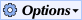
\includegraphics[width=2.1cm]{options_button.png}}\\Options menu button
  \end{framed}
\end{wrapfigure}
Click on the ``Options'' menu button to open up the gene entry's menu.
If you do not see the ``Options'' menu button, you are not logged in or you do not have rights to edit this gene's settings.
In the opened menu, click ``Edit gene information'' to open up the gene's edit form.
The fields on the form are explained in the section ``\hyperlink{s_gene_create}{Creating a new gene database}''.
After you submit the form, LOVD redirects you automatically back to the gene's homepage.





\section{Deleting a gene database}
\begin{wrapfigure}[3]{r}{8cm} % Only wrap for 3 lines
  \vspace{-25pt}
  \begin{leftbar}
    Required level: Manager\\
    Available from: LOVD 3.0 Build 01
  \end{leftbar}
\end{wrapfigure}
Only managers and up can delete gene databases from LOVD.
To delete the gene database in question, first proceed to the \hyperlink{s_gene_homepage}{gene's homepage}.
Click on the ``Options'' menu button to open up the gene entry's menu, and select the ``Delete gene entry'' option.
To complete the removal, you need to fill in your password and submit the form.

\begin{warntable}
Removing a gene can not be undone, you will need to create the gene database again.
% TODO: when we have import...
%If in any doubt, first make a download of the database so that you can re-upload the data .....blabla
Please note that deleting a gene removes also its transcripts in the database and therefore all variant annotation on the gene in question, but it \emph{does not remove the genomic variants from the database}.
%TODO: so how do we delete these variants?
\end{warntable}





\hypertarget{s_gene_assign_curators}{}
\section{Assigning curators and collaborators}
\begin{wrapfigure}[3]{r}{8cm} % Only wrap for 3 lines
  \vspace{-25pt}
  \begin{leftbar}
    Required level: Manager\\
    Available from: LOVD 3.0 Build 01
  \end{leftbar}
\end{wrapfigure}
...
%You can set an authorized user as a gene curator by editing the user's account and selecting the relevant genes in the "Curator for" field.
















\end{document}

%            s (section) ss (subsection)
\hypertarget{s_name_of_label}{}
\hyperlink{name_of_label}{name of link}.

\begin{infobox}
  \caption{\textbf{Caption}}
  ...
\end{infobox}

% Add to text explaining how to log in:
Cookies are small text files stored on your computer that help a website identify you. LOVD uses this to keep you identified after you log into the system. If this setting is disabled, LOVD will include a so-called session id in the URL, to keep track of the authenticated users. However, this is much less secure because including the session id in the URL may expose this session id in log files on your computer or on proxy servers. This may allow others to hijack your user's accounts. So leaving this option set is highly recommended.

% Maybe move to create individual?
List of possible diseases associated with variants in the available genes: Specify a list of phenotypes that are used in this LOVD installation. This list will appear on the full legend and will allow a submitter to select a phenotype from the list. If no phenotypes are specified, the submitter will need to fill in the phenotype in a common text field.

% Move somewhere about the screening data:
List of available detection techniques: Specify a list of detection techniques appropriate for the genes configured in this LOVD installation. By default, a full set of detection techniques has been put in this list already. This list will appear on the full legend and will allow a submitter to select the used detections technique(s) from the list. If no techniques are specified, the submitter will need to fill in the technique in a common text field.

%10
\chapter{}
%5
\section{}
%3
\subsection{}
%1
\subsubsection{}



$_PAGES =
     array(
            'LOVD Setup',
             array(
                    'Gene databases',
                     array(
                            'Emptying genes',
                          ),
                    'Custom columns',
                     array(
                            'Variant vs. patient columns',
                            'Managing patient columns',
                            'Creating new columns',
                            'Editing custom column default settings',
                            'Deleting custom columns',
                            'Downloading custom column data to text files',
                            'Importing custom columns from text files',
                          ),
                    'Custom links',
                     array(
                            'Creating new links',
                            'Editing links',
                            'Deleting links',
                          ),
                    'Modules',
                     array(
                            'Installing modules',
                            'Enabling or disabling modules',
                            'Uninstalling modules',
                            'Available LOVD modules',
                          ),
                  ),
            'LOVD Gene configuration area',
             array(
                    'Gene settings',
                    'Custom variant columns',
                    'Curating variants',
                    'Download or import variants',
                    'Advanced edit features',
                     array(
                            'Find & Replace',
                            'Copy Column',
                          ),
                  ),
            'Gene homepage',
             array(
                    'News feed',
                  ),
            'Variant and patient data',
             array(
                    'Viewing and searching variant and patient data',
                     array(
                            'Advanced options',
                          ),
                    'Submitting variant and patient data',
                    'Editing variant data',
                    'Editing patient data',
                    'Deleting variant or patient data',
                    'Downloading data to text files',
                    'Importing text files',
                    'Database statistics',
                  ),
            'Submitters',
             array(
                    'Registering a new account',
                    'Keeping your account up to date',
                    'Keeping track of your submissions',
                  ),
            'LOVD scripts',
             array(
                    'Enabling the scripts',
                    'GenBank File Uploader',
                    'Reading Frame Checker',
                    'Reference Sequence Parser',
                  ),
            'Use of HTML within LOVD',
            'Updating LOVD',
            'Keeping your data secure',
          );




(couldn't get color into this one...)

\usepackage{fancybox} % New attempt for fancy boxes...

\newlength{\mylength}
\newenvironment{infotable}%
{\setlength{\fboxsep}{15pt}
\setlength{\mylength}{\linewidth}%
\addtolength{\mylength}{-2\fboxsep}%
\addtolength{\mylength}{-2\fboxrule}%
\addtolength{\mylength}{-1.5cm}%
\Sbox
\begin{minipage}[t]{1.5cm}

\includegraphics[width=1cm]{lovd_information.png}
\end{minipage}
\minipage{\mylength}%
}%
{\endminipage\endSbox
\[\fbox{\TheSbox}\]}


